
\chapter{État de l'art }



\section*{Introduction }
Dans ce chapitre, nous nous penchons sur les fondements de la connectivité réseau en étudiant les technologies établies telles que les MPLS et les VPNs . Nous examinons leurs fonctionnements et leurs architectures. En outre, nous abordons les défis rencontrés, en particulier en termes de flexibilité et de coût. Enfin, nous introduisons la solution SD-WAN comme une alternative prometteuse pour répondre aux besoins évolutifs des réseaux modernes.

\section{Etudes de l'éxistant }
\subsection{Mpls }
\subsubsection{Généralité sur mpls }
\begin{itemize}
	\item[$\bullet$]\textbf{Définition:} 
	
	MPLS, acronyme de Multiprotocol Label Switching, a été initialement introduit dans les années 1970 par plusieurs ingénieurs Internet pour résoudre diverses problématiques d'Internet, principalement en ce qui concerne les performances de routage, dans lesquelles l'en-tête de chaque paquet devait être lu et analysé avant d'être envoyé vers la bonne destination. Après près de 20 ans de lutte et de développement, MPLS a finalement été reconnu et confirmé par l'IETF (Internet Engineering Task Force) à la fin des années 1990, devenant ainsi une norme ouverte prête à être adoptée. De plus en plus adoptée par les fournisseurs de services dans leurs infrastructures principales, MPLS s'intègre aux protocoles de couche 2 et de couche 3.

\end{itemize}
\begin{itemize}
	\item[$\bullet$]\textbf{L'en-tête MPLS :} 
	
L'en-tête MPLS a une longueur de 32 bits comme montre la figure.
\begin{figure} [H]
	\begin{center}
		\centering
		\hspace*{-0.5cm}
		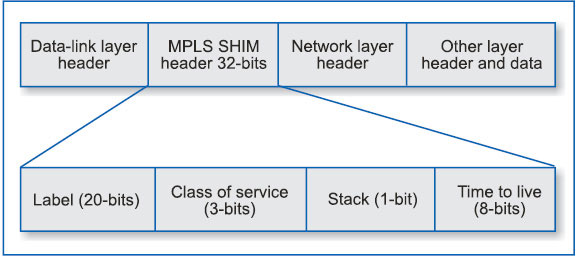
\includegraphics[width=0.67\linewidth]{Images/mpls entete}
	\end{center}
	\caption{Entête MPLS}
\end{figure} 

Le champ d'étiquette est de 20 bits, et ces étiquettes sont attachées aux paquets au point d'entrée dans un réseau MPLS. 

Dans le réseau, les étiquettes sont utilisées pour router les paquets sans tenir compte des informations d'en-tête originales des paquets. Elles peuvent être empilées comme une pile LIFO, ce qui permet à MPLS d'être utilisé pour le transport et la distribution.

Le champ CoS (Class of Service) est de 3 bits. Il affecte les algorithmes de planification et/ou de suppression appliqués au paquet lors de sa transmission à travers le réseau. Ces bits ne sont pas modifiés par l'implémentation embarquée de MPLS.
Le bit Stack est défini à 1 pour la dernière entrée dans la pile d'étiquettes et à 0 pour toutes les autres entrées de pile d'étiquettes.

Le champ TTL (Time To Live) est de 8 bits. Il est décrémenté de 1 chaque fois que le paquet passe par un routeur. Le paquet est supprimé lorsque le TTL atteint zéro. 
	
\end{itemize}
\subsubsection{Architecture d'un réseau MPLS de base }
C’est une architecture qui fait référence à une mise en œuvre simple et directe de MPLS, où les routeurs MPLS sont utilisés pour acheminer les paquets en fonction des étiquettes MPLS sans ajouter de couches ou de fonctionnalités supplémentaires, comme le montre la Figure.
\begin{figure} [H]
	\begin{center}
		\centering
		\hspace*{-0.5cm}
		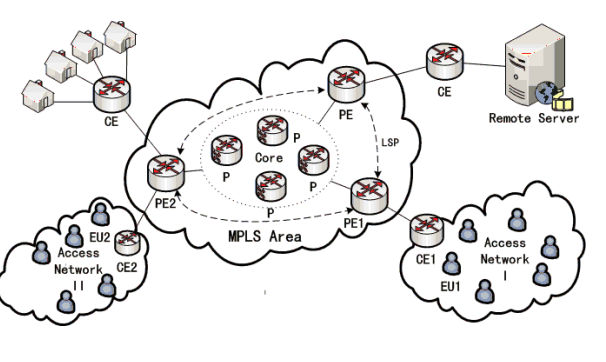
\includegraphics[width=0.67\linewidth]{Images/architecture-mpls}
	\end{center}
	\caption{Architecture du réseau mpls}
\end{figure} 


On trouve trois types différents de routeurs dans l'architecture de réseau MPLS : les routeurs PE et les routeurs P qui sont activés pour MPLS, et les routeurs CE qui sont des routeurs réguliers d'accès. Le routeur P est utilisé dans la zone centrale, son rôle principal est d’acheminer les paquets de données étiquetés tandis que le routeur PE est utilisé pour l'encapsulation et la désencapsulation des données ainsi que pour faire la liaison entre les routeurs P et CE.

Les routeurs PE fonctionnent avec deux types différents de routage : le premier protocole s’applique entre PE et CE pour modifier les informations d’adresse IP et de connexion tandis que le deuxième protocole s’applique au sein de la communication entre P et PE pour distribuer des étiquettes et gérer les LSP (chemins de distribution d’étiquettes).
 \subsubsection{Mécanisme de transfert de données dans une architecture de réseau MPLS de base  }
 La procédure de transfert de données entre deux utilisateurs dans deux réseaux d'accès différents est décrite comme suit,les paquets IP sont envoyés à CE, qui vérifie ensuite l'adresse de destination et recherche dans sa table de routage pour déterminer si les paquets de données doivent être transmis à un PE ou à d'autres utilisateurs dans le même réseau d'accès. 
 
 Ensuite, les paquets sont envoyés jusqu'au PE, qui vérifie à nouveau l'adresse de destination et choisit les étiquettes correspondantes à ajouter aux paquets en fonction de sa base de données FEC (Classe d'Équivalence de Transfert). La FEC assure le stockage de la relation de mappage entre les étiquettes sortantes et certaines adresses de destination.
  
  Après l'encapsulation, les paquets de données étiquetés sont envoyés aux routeurs P pour un acheminement rapide dans la zone centrale. Chaque saut pour un paquet de données dans la zone MPLS doit être accompagné d'un commutation d'étiquette. Après avoir suivi la route prédéfini et traversé la zone centrale, les paquets étiquetés arrivent au PE où ils sont désencapsulés et transférés à CE, qui vérifie ensuite l'adresse de destination et envoie le paquet de données à l'utilisateur.
  \subsection{VPN}
  \subsubsection{Définition }
  Un VPN est un réseau privé construit au sein d'une infrastructure de réseau public, telle que l'Internet. Il permet à des utilisateurs distants de se connecter de manière sécurisée en créant un tunnel crypté entre l'appareil de l'utilisateur et le réseau privé. Cette méthode assure la confidentialité et la sécurité des données échangées. Le VPN permet aux utilisateurs d'accéder aux ressources du réseau privé, telles que des fichiers, des applications et des imprimantes, comme s'ils étaient physiquement connectés au réseau local.      
  
  \subsubsection{les technologies VPN  }
  \begin{itemize}
  	\item[$\bullet$]\textbf{ IPSec :} 
  	
  	IPSec est appliqué au niveau de la couche réseau sans être en combinaison avec d'autres protocoles. Il fournit une collection de protocoles normalisés et de techniques pour établir des connexions VPN sécurisées. En assurant l’authentification, l’encapsulation et l’intégrité des paquets, IPSec garantit la sécurité des données. De plus, il peut établir des tunnels VPN entre des passerelles IPSec de différents fabricants grâce à sa normalisation. Bien que IPSec détermine les méthodes et les protocoles d'échange de base, il ne spécifie pas le niveau de sécurité à utiliser.
  	
  	Il existe deux modes de base de connexions IPSec. Dans le mode transport, un en-tête IPSec est ajouté à l'en-tête IP d'origine, contenant des informations d'authentification et d'intégrité. En revanche, dans le mode tunnel, chaque paquet IP d'origine est entouré d'un nouveau paquet IP comprenant un nouvel en-tête IP et l'en-tête IPSec. Ainsi, les informations sur le contenu du paquet IP d'origine sont cachées dans la charge utile du nouveau paquet IP.
  	
  	Lors de l'établissement d'une connexion IPSec, il y a deux phases de négociation. Pendant la première phase, la SA pour IKE est négociée, sans chiffrement ni authentification de données. Par contre, les deux partenaires doivent s'authentifier et échanger les clés en utilisant l'algorithme de chiffrement asymétrique à clé publique, Diffie-Hellman. Une fois les clés échangées, la phase deux est initiée. Pendant cette phase, déjà protégée, les paramètres des tunnels VPN sont négociés, y compris les clés de chiffrement symétriques, les informations d'expiration des clés, la politique de sécurité et les routes réseau. Après cela, les données peuvent être échangées de manière sécurisée.
  \end{itemize}
    \begin{itemize}
  	\item[$\bullet$]\textbf{L2TP :} 
  	
  	L2TP est le protocole de tunnelisation appliqué au niveau de la couche de liaison de données, il est basé sur le protocole de transfert L2F(Layer Two Forwarding), Il permet d'encapsuler une trame de la couche de liaison de données complète dans un paquet UDP au niveau de transport. Ce paquet UDP, transportant la trame de la couche deux, comprend plusieurs champs de données ,on trouve une en-tête UDP, des bits de contrôle représentant diverses options, la version et la longueur du paquet.
  	
  	 Ensuite, les champs de numéro de séquence et d'identifiant de tunnel qui permettent de suivre la connexion VPN actuelle pour assurer le traitement correct des paquets.
  	 
  	  Enfin, la trame de la couche deux qui contient des éléments tels que les adresses de contrôle d'accès au support (MAC) et la charge utile.
  	Pour garantir l'authentification et la confidentialité, l'encapsulation seule d'une trame de couche deux dans un paquet UDP n'est pas suffisante. C'est pourquoi le L2TP est souvent combiné avec IPSec en mode transport, en ajoutant l'en-tête IPSec devant l'en-tête L2TP. 
  \end{itemize}
     \begin{itemize}
  	\item[$\bullet$]\textbf{PPTP:} 
  	
  Le protocole de tunnelisation point-à-point de Microsoft est une extension du protocole point-à-point (PPP) et est pris en charge par toutes les versions de Microsoft Windows. 
  
  Pour établir une connexion VPN, PPTP utilise deux types différents de paquets , on trouve les paquets GRE (Generic Routing Encapsulation) qui transportent la charge utile du VPN en ajoutant l’en-tête GRE au paquet d’origine. L’en-tête GRE est assez similaire à l’en-tête L2TP et contient divers bits de contrôle, numéros de séquence et de tunnel. On trouve aussi les messages de contrôle PPTP, qui sont simplement des paquets TCP contenant des informations de contrôle telles que les demandes et réponses de connexion, les paramètres de connexion et les messages d'erreur.
  
  Microsoft utilise le protocole d'authentification par challenge (MS-CHAP) pour authentifier les deux partenaires de tunnel, car ni GRE ni les messages PPTP ne fournissent d'authentification ou de chiffrement.
 
  PPTP peut être utilisé pour établir des connexions VPN entre les réseaux des fournisseurs de services Internet et leurs clients, qui n'ont pas besoin d'installer de logiciel VPN supplémentaire. 
  \end{itemize}
  \subsection{les connexions dédiées}
  
  Les lignes dédiées ou spécialisées sont des connexions point à point ou multipoint qui permettent la transmission de données à des débits moyens et élevés. Ces connexions offrent une bande passante garantie et une faible latence, ce qui les rend idéales pour les applications qui nécessitent une communication rapide et fiable entre des sites distants.
 
  Les premiers liens numériques dédiés ont été développés dans les années 1970.  On parle du lien T1 comme un exemple , il utilise deux paires torsadées pour transmettre à des débits allant jusqu'à 1,544 Mbit/s dans les deux sens (avec 24 canaux vocaux). De manière similaire, le lien E1 offre une bande passante de 2,048 Mbit/s (avec 32 canaux vocaux). Ces types de connexions sont couramment utilisés pour relier des réseaux locaux (LAN) distants.
  
  Pour les connexions à longue distance, des câbles coaxiaux sont souvent utilisés, avec des répéteurs disposés tous les 60 kilomètres environ. Ces répéteurs sont nécessaires pour régénérer le signal et maintenir la qualité de la transmission sur de longues distances.
  En résumé, les lignes dédiées fournissent une connectivité haut débit et fiable entre des sites distants, ce qui en fait un choix privilégié pour les entreprises et les organisations qui ont besoin d'une communication stable et rapide entre leurs différentes implantations.
  \subsection{les réseaux Frame Relay}
  Le réseau Frame Relay est une technologie largement utilisée dans les années 1990 et au début des années 2000 pour connecter des sites distants via des connexions de réseau à commutation de paquets.
  
  Le principe du Frame Relay est de découper les données en petits paquets appelés "frames" et de les transmettre sur le réseau en utilisant des circuits virtuels. Ces circuits virtuels étaient établis entre les sites distants et étaient gérés par les équipements du fournisseur de services. Chaque paquet (ou frame) contient une étiquette d'identification qui permettait au réseau de router le paquet vers sa destination appropriée.
  
  Les réseaux Frame Relay offrent plusieurs avantages par rapport aux lignes dédiées traditionnelles. Tout d'abord, ils sont plus flexibles car ils permettent de partager une même liaison entre plusieurs sites distants . De plus, les circuits virtuels pouvaient être configurés et reconfigurés rapidement en fonction des besoins de l'entreprise, offrant ainsi une grande souplesse.
  \subsection{Les réseaux ATM }
  
  Les réseaux ATM (Asynchronous Transfer Mode) est une technologie largement déployée dans les années 1990 et au début des années 2000. Contrairement au Frame Relay, qui repose sur la commutation de paquets, l'ATM est basé sur la commutation de cellules. Chaque cellule ATM avait une taille fixe de 53 octets, ce qui assure un traitement plus efficace et prévisible du trafic.
  
  Les réseaux ATM sont utilisés pour transporter le trafic généré par une grande variété d'applications, chacune ayant des caractéristiques de trafic et des exigences de performances réseau différentes. 
  Pour répondre efficacement à cet environnement multi-applications, la couche ATM définissait un ensemble sophistiqué de fonctions et de procédures de gestion du trafic.
  Parmi les principaux objectifs de ces fonctions et procédures de gestion du trafic de la couche ATM, on peut citer :
  \begin{itemize}
  \item Protéger le réseau et les utilisateurs afin d'atteindre les objectifs de performance du réseau.
  \item Optimiser l'utilisation des ressources du réseau.
  \item Protéger les applications contre la congestion du réseau.
\end{itemize}
\section{Problématique}

Dans un monde où les entreprises évoluent rapidement, la nécessité d'une connectivité réseau agile et flexible est devenue indisponsable surtout dans le milieu militaire . 
Les solutions traditionnelles de mise en réseau peinent souvent à répondre aux exigences changeantes des entreprises, entraînant des inefficacités opérationnelles et des coûts élevés. 

Tout d'abord, les réseaux Frame Relay et ATM ont été critiqués pour leur manque de flexibilité et d’ Adaptabilité . la Configuration et la reconfiguration des circuits virtuels dans un réseau Frame Relay, par exemple, pouvait être Pénible et nécessite souvent l'intervention du fournisseur de services, ce qui entraîne des délais et des coûts supplémentaires.

De plus, ces technologies étaient souvent limitées en termes de bande passante et ne pouvaient pas toujours s'adapter efficacement aux besoins changeants des entreprises, en particulier avec l'émergence de nouvelles applications gourmandes en bande passante telles que la vidéoconférence et la VoIP.

Les connexions dédiées, bien qu'elles garantissent une bande passante stable et une faible latence, peuvent être coûteuses à mettre en place et à entretenir, notamment pour les déploiements multi-sites dans le domaine militaire. 
face aux défis posés par les infrastructures réseau traditionnelles, il est impératif de rechercher des solutions innovantes qui révolutionne la façon dont les entreprises gèrent leur infrastructure réseau ,une approche qui offre une connectivité robuste et évolutive tout en simplifiant la gestion globale du réseau.

Tout d'abord, on parle d’une connectivité multicloud, permettant aux entreprises de tirer parti de multiples fournisseurs de services cloud sans compromettre la performance ou la sécurité. Cette capacité à intégrer facilement des services cloud dans l'infrastructure réseau offre une flexibilité et une agilité exceptionnelles. elle permet aux entreprises de s'adapter rapidement aux changements du marché et aux nouvelles exigences métier.
De plus, une utilisation efficace des ressources réseau en tirant parti de la diversité des chemins de données disponibles, qu'il s'agisse de connexions Internet, de liaisons MPLS ou d'autres types de connexions. En équilibrant intelligemment le trafic sur ces différents chemins, on garantit une performance optimale et une disponibilité élevée, même dans des conditions de réseau variables. Cette capacité à optimiser la bande passante disponible est essentielle pour répondre aux besoins croissants en termes de volume de données et d'applications gourmandes en bande passante.

La sécurisation des communications réseau revêt aussi une importance majeure en offrant un chiffrement de bout en bout et des fonctionnalités avancées de pare-feu et de prévention des intrusions. En sécurisant les communications réseau à tous les niveaux, on garantit la confidentialité et l'intégrité des données, même lorsqu’on traverse des réseaux non sécurisés comme Internet. Cette sécurité renforcée est particulièrement importante dans un environnement où les cybermenaces sont de plus en plus sophistiquées et omniprésentes.

Enfin, la simplification de la gestion globale du réseau en offrant une interface centralisée et intuitive pour la configuration, la surveillance et le dépannage. En consolidant les opérations réseau dans une seule plateforme, on  réduit la complexité et les coûts associés à la gestion de multiples appareils et systèmes.Cette simplification de la gestion est essentielle pour décharger les équipes informatiques des tâches fatigantes, leur permettant ainsi de se concentrer pleinement sur des initiatives stratégiques à forte valeur ajoutée.
\section{Solution proposé }

Face à la nécessité croissante d'une infrastructure réseau agile et flexible, les solutions traditionnelles rencontrent souvent des difficultés pour s'adapter aux exigences évolutives et complexes.C'est dans ce contexte que les technologies de Software-Defined Networking (SDN) émerge comme l’un des solutions innovantes , offrant des perspectives nouvelles pour la gestion et l'optimisation des réseaux d'entreprise.

\subsection{Généralité sur SDN }

Le réseau défini par logiciel (SDN ) est une approche innovante pour concevoir, mettre en œuvre et gérer des réseaux qui séparent le contrôle du réseau (plan de contrôle) et le processus de transfert de données (plan de données) pour une meilleure expérience utilisateur.
SDN facilite le déploiement d'applications au sein des organisations et permet une livraison flexible . De plus il offre la capacité de mettre à l'échelle les ressources réseau en parallèle avec les besoins des applications et des données, et réduisant à la fois les dépenses en capital (CapEX) et les dépenses opérationnelles (OpEX). 
\subsection{Architecture du SDN   }
L'architecture du SDN (Software-Defined Networking) est divisée verticalement en trois couches comme montre la figure.

\begin{figure} [H]
	  \hspace{0.9cm}
	\begin{center}
        \centering
		\hspace*{-0.5cm}
		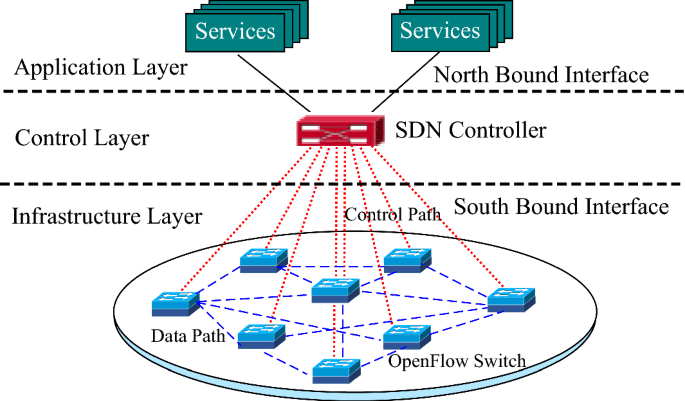
\includegraphics[width=0.67\linewidth]{Images/SDN-arch}
	\end{center}
	\caption{Architecture du SDN}
\end{figure} 
\subsubsection{Couche d'infrastructure }

C'est la couche inférieure qui comprend les commutateurs, les routeurs et d'autres périphériques réseau physiques. Ces périphériques, appelés des éléments de commutation, sont chargés de transférer les paquets et sont responsables de l'acheminement réel du trafic en fonction des instructions fournies par la couche de contrôle.

Dans le contexte du SDN, la séparation entre le contrôle et le plan de données exige que le plan de données soit accessible à distance pour un contrôle basé sur un logiciel via une interface Sud (Southbound interface) ouverte et indépendante du fournisseur.
\subsubsection{Couche de contrôle }

Cette couche est responsable de la logique de contrôle du réseau et est considérée comme l'entité fondamentale dans l'architecture SDN. Elle comprend un contrôleur logiciel centralisé chargé de gérer les communications entre les applications réseau et les appareils via des interfaces ouvertes.

La couche de contrôle SDN est souvent appelée le système d'exploitation réseau (NOS) car elle prend en charge la logique de contrôle du réseau et fournit à la couche d'application une vue abstraite du réseau global, contenant suffisamment d'informations pour spécifier des politiques tout en masquant tous les détails de mise en œuvre.

Dans une configuration de contrôle SDN distribué, des APIs Est-Ouest sont nécessaires pour permettre à plusieurs contrôleurs SDN de communiquer entre eux et d'échanger des informations réseau. 

\subsubsection{Couche d'application }

C'est la couche supérieure où résident les applications et les services réseau qui sont des programmes de contrôle conçus pour mettre en œuvre la logique et les stratégies de contrôle du réseau. Cette couche de niveau supérieur interagit avec la couche de contrôle via une API Nord ouverte.Ainsi, les applications SDN communiquent leurs besoins réseau au contrôleur SDN qui les traduit en commandes spécifiques au Sud et en règles de transfert dictant le comportement des périphériques de plan de données individuels.

Le routage, l'ingénierie du trafic (TE), les pare-feu et l'équilibrage de charge sont des exemples d'applications SDN courantes s'exécutant sur les plates-formes de contrôle existantes . 
\subsection{la solution SD-wan  }
aprés avoir explorer en profondeur l'architecture et les fonctionnalités du SDN, il est important de souligner que le SD-WAN(Software-Defined Wide Area Network), émerge comme une évolution naturelle de cette technologie révolutionnaire.

Le SD-WAN tire parti des fondements du SDN en séparant le plan de contrôle du plan de données, permettant ainsi une gestion centralisée et une adaptation dynamique du trafic sur des réseaux étendus. En intégrant des fonctionnalités avancées telles que le routage intelligent, la gestion dynamique des liens, et la qualité de service (QoS) basée sur les applications, le SD-WAN offre une agilité et une flexibilité accrues pour répondre aux besoins changeants des entreprises en matière de connectivité réseau.

\section*{Conclusion }

Dans ce premier chappitre ,nous avons examiné attentivement l'étude de l'existant, identifié la problématique associée et présenté une première approche de solution. Dans le chapitre suivant, nous passerons à une analyse plus détaillée et à une spécification approfondie des besoins, afin de mieux comprendre les exigences spécifiques et les objectifs à atteindre dans le cadre de notre projet.